% !TeX root = ../main.tex

\chapter{面向性能预测的着色器性能数据集}
\label{sec:perf_data_set_chap}

{\added 本章提出了面向性能预测的着色器性能数据集。渲染中的着色器程序的性能收集和理解面临多种挑战,本章的引言部分将首先介绍数据集工作面临的问题。之后,本章将详细介绍着色器收集和性能测量部分的实现。同时,为了更好的了解着色器程序本身的功能类型特征,本章同时将介绍一种使用基座语言模型来进行着色器类型标注的相关尝试。最后,本章将通过实验和分析验证本章提出的数据集的质量和分布信息。}

\section{{\amend 引言}}

{\amend 着色器程序是利用 GPU 进行实时渲染的过程中,嵌入到绘制流水线中的程序片段。由于性能对于游戏等实时渲染程序来说至关重要,故而了解着色器程序的性能对于程序的优化来说可以起到一定的帮助。对于数据驱动的着色器程序性能预测方法来说,高质量的着色器程序性能数据是其成功的关键。同时,不同类型的着色器程序可能在不同平台上体现不同的性能特征,这些行为也需要跨越不同平台的着色器性能数据集加以刻画。然而,构建这样的数据集面临着如下挑战:

{\bf 其一},尚无用于着色器程序性能理解和学习的公开着色器性能数据集。经典的程序语言理解数据集,如其中包含 POJ-104 \cite{10.5555/3015812.3016002}、GitHub Java Corpus 等的 CodeXGLUE 数据集\cite{DBLP:journals/corr/abs-2102-04664},更多关注于代码的通用语义理解,而对性能部分关注较少。GPU 上的数据集,如 OpenCL 异构映射任务数据集\cite{8091247},则多只关注于通用计算方面,且程序的规模和丰富程度均需要进一步增强。

% TODO: 如果第二章基础知识部分增加了相关的说明,可以挪动到这里。
{\bf 其二},着色器程序的性能受到多种波动的影响,而现有的程序理解数据集中,多只有简单的运行时间,缺乏对于运行时间的稳定度的分析。例如,面向机器学习的大规模程序理解数据集 CodeNet \cite{DBLP:journals/corr/abs-2105-12655} 中,关于程序性能的标注只有 CPU 运行时间和运行内存两项。对于 GPU 上运行的程序来说,整个计算过程经过的环节更多,所以运行时间的不确定性也会更强。}

{\added{\bf 其三},着色器程序实现的效果多种多样,而程序的类型对于后续的理解工作会起到一定作用。例如,仅仅在片段着色器程序中,程序开发者就可以实现图 \ref{fig:shadertoy_gallery_ch3} 中多样的画面效果。程序开发者通常会在代码内和平台上留有一定程度的作品标签信息,如本章使用的数据来源 Shadertoy 平台就提供向上传作品的属性信息中添加 tag 的功能。然而,许多上传的着色器程序,其标注并不完备。

\begin{figure}[htbp]
  \centering
  \begin{minipage}[b]{\textwidth}
      \begin{subfigure}[b]{0.48\textwidth}
          
\includegraphics[width=\textwidth]{figures/shadertoy_cloud.png}
          \caption{过程化纹理生成 (PTG)}
          \label{fig:sub_textgen}
      \end{subfigure}
      \hfill % Adds horizontal space between the subfigures
      \begin{subfigure}[b]{0.48\textwidth}
          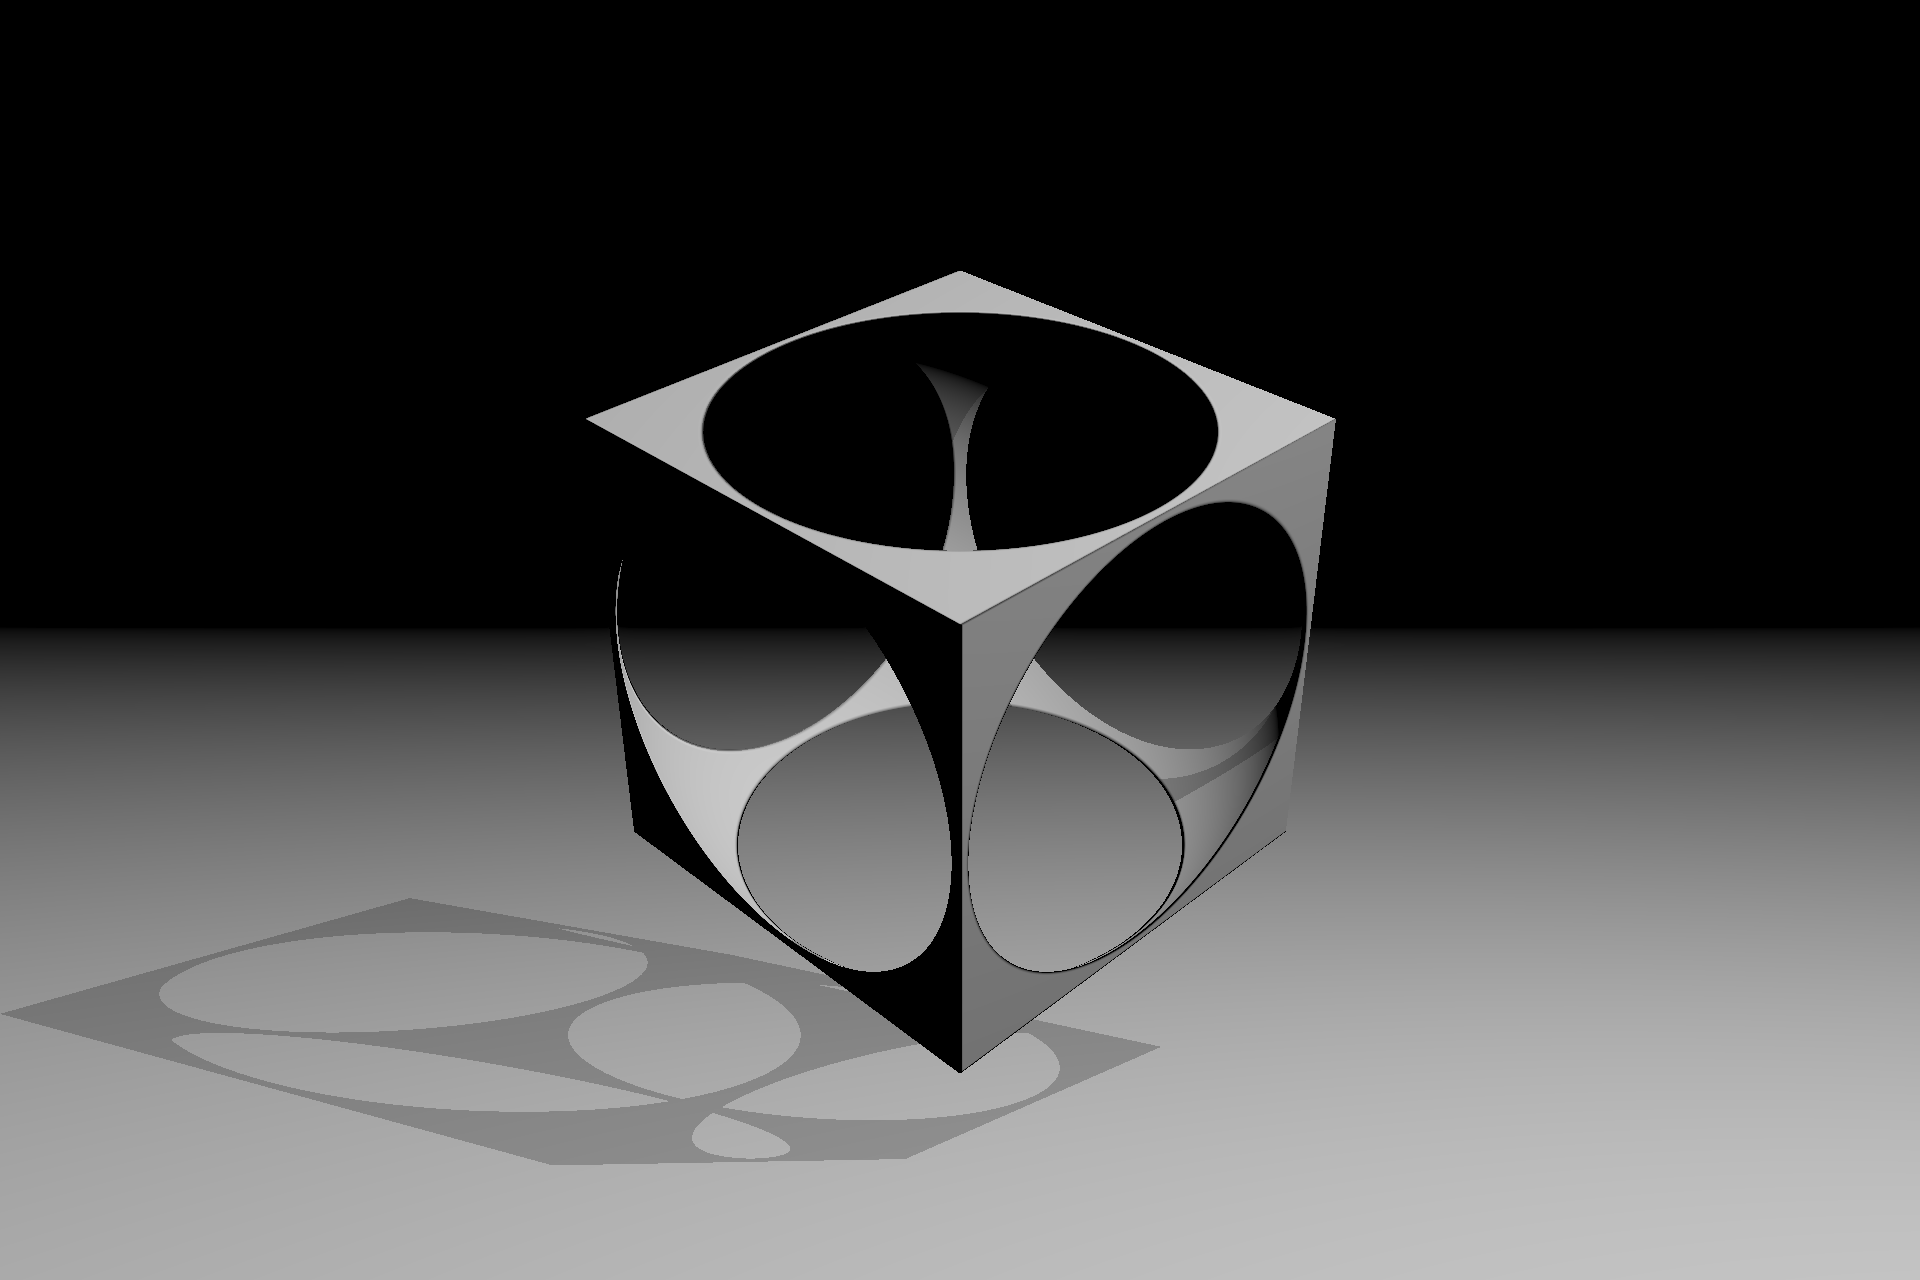
\includegraphics[width=\textwidth]{figures/shadertoy_csg.png}
          \caption{构造实体几何 (CSG)}
          \label{fig:sub_csg}
      \end{subfigure}
  \end{minipage}
  
  %\vspace{1em} % Adds vertical space between the rows of subfigures
  
  \begin{minipage}[b]{\textwidth}
      \begin{subfigure}[b]{0.48\textwidth}
          
\includegraphics[width=\textwidth]{figures/shadertoy_raymarching.png}
          \caption{光线步进 (Ray Marching)}
          \label{fig:sub_raymarching}
      \end{subfigure}
      \hfill % Adds horizontal space between the subfigures
      \begin{subfigure}[b]{0.48\textwidth}
          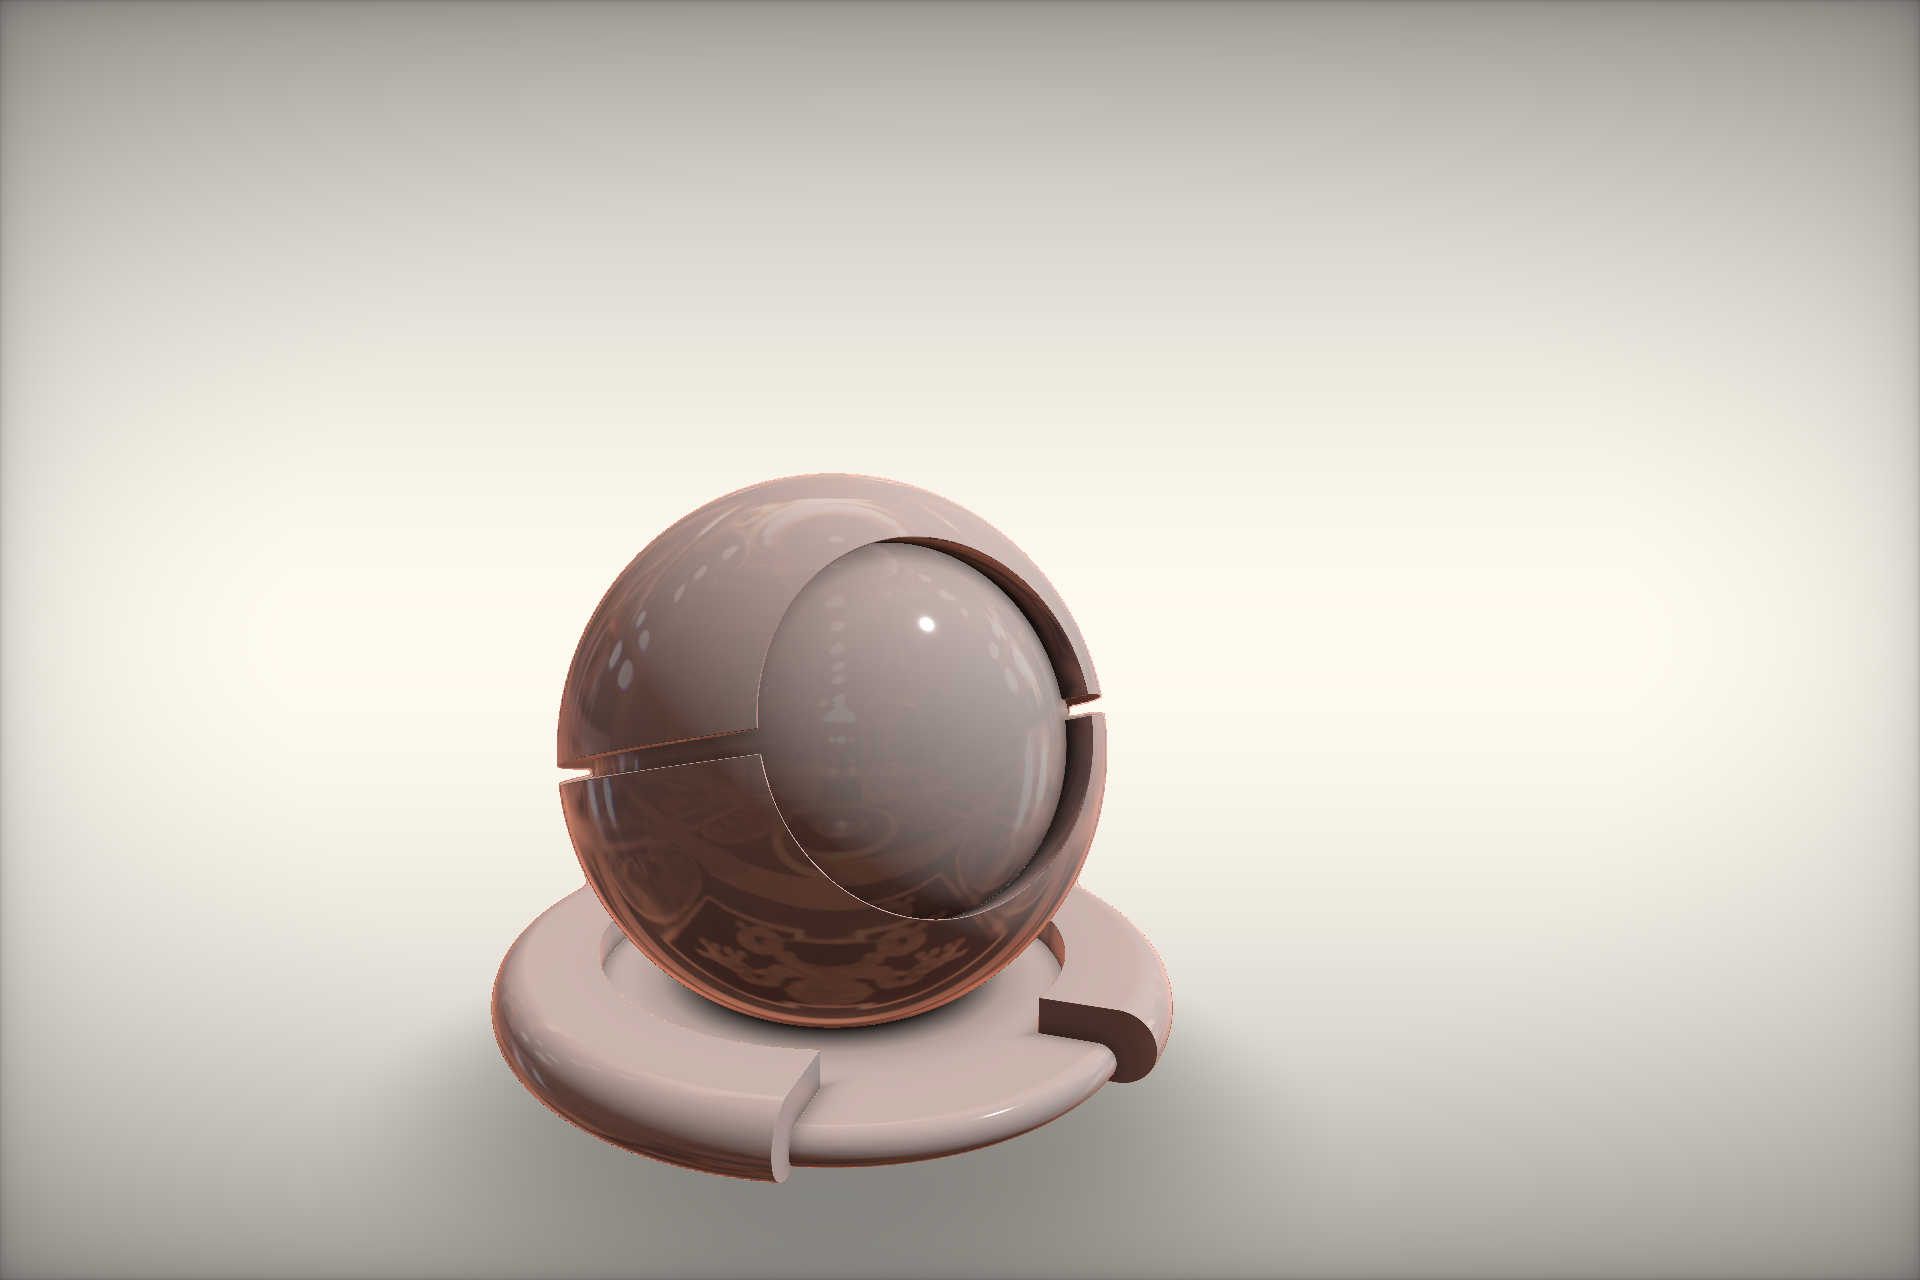
\includegraphics[width=\textwidth]{figures/shadertoy_pbr.png}
          \caption{基于物理的着色 (PBS)}
          \label{fig:sub_pbs}
      \end{subfigure}
  \end{minipage}
  
  \caption{Shadertoy 用户\cite{ShdrToyUser1, ShdrToyUser2}着色器程序效果示例与其使用的主要技术}
  \label{fig:shadertoy_gallery_ch3}
\end{figure}


本章提出的数据集将基本解决上述问题。针对问题一,本章所描述的方法构造了新的着色器性能数据集,其包含 5 个 GPU 平台,共 54667 个片段着色器性能样本。针对问题二,本章性能测量时使用了重复采样和 GPU 端时间戳测量,并在实验时对样本的变异系数进行了分析。}{\added 针对问题三,本章探索了利用基座语言模型、结合人工进行半自动着色器类型标注的相关方法,为着色器数据集内的功能类型提供了参考。同时,本章提出的数据集将进一步给出在不同平台间有显著性能相对差异的着色器挑战样本集合。并在实验部分给出数据集的质量评估。
}

\section{{\amend 着色器收集和性能测量}}

{\added 本章提出的数据集的数据来源于 Shadertoy\cite{Shadertoy} 网站上用户上传的着色器程序数据。} Shadertoy 是一个在线{\added 的着色器共享}平台,{\amend 其}允许用户创建、分享和查看着色器程序{\amend 并在线查看}渲染结果。

{\added 对于 GPU 上基于光栅化的图形渲染程序来说,其通常需要}指定管线的顶点和三角面索引输入,同时给出过程中用到的顶点、片元等着色器{\amend 以调用 GPU 进行绘制操作。}不过,出于降低上手门槛、让用户专注于创造新奇有趣的视觉效果本身的考虑,Shadertoy 平台上在进行显示绘制时,均{\amend 使用输入图元为覆盖全视口的两个三角形作为输入,且使用一个在顶点变换阶段原样输出的顶点着色器。}{\added 该着色器可以使用 WebGL Inspector \cite{WebGLInspector} 截出。}

作为示例,一个简单的 Shadertoy 着色器如图 \ref{fig:example_glsl_shadertoy_code_ch3} 中代码所示,其渲染结果如图 \ref{fig:example_shadertoy_output_ch3} 所示。

\begin{figure}  % 'h' for here, 't' for top, 'b' for bottom, 'p' for on a separate page
\centering

\begin{lstlisting}[language=GLSL]
void mainImage( out vec4 fragColor, in vec2 fragCoord )
{
    // 从 0 到 1 的归一化屏幕坐标
    vec2 uv = fragCoord/iResolution.xy;

    // 生成随时间 iTime 变化的像素颜色
    vec3 col = 0.5 + 0.5*cos(iTime+uv.xyx+vec3(0,1,5));

    // 输出到屏幕
    fragColor = vec4(col,1.0);
}
\end{lstlisting}
\caption{在屏幕上产生渐变颜色的 Shadertoy 代码示例}
\label{fig:example_glsl_shadertoy_code_ch3}
\end{figure}

\begin{figure}
  \centering
  
\includegraphics[width=0.65\textwidth]{figures/example_shadertoy_output.png}
  \caption{在屏幕上产生渐变颜色的 Shadertoy 效果示例}
  \label{fig:example_shadertoy_output_ch3}
\end{figure}

如图 \ref{fig:shadertoy_gallery_ch3},尽管在渲染时缺乏多样的几何输入,{\amend Shadertoy 上的着色器程序}仍然可以通过应用如光线步进(Ray Marching)\cite{Hart1996}, 过程化内容生成(Procedural Content Generation)等技术来创建能够产生复杂视觉效果的着色器。Shadertoy 网站收集的着色器在渲染技术方面覆盖相当完备{\amend 负载情况变化多样},故而{\amend 本章}以 Shadertoy 上的着色器为基础,构建片元着色器性能数据集。

\subsection{数据收集}

为了方便第三方程序的编写,Shadertoy 网站提供了基于 HTTP GET 的 API 接口,这为{\amend 数据集构建过程中的}数据收集工作提供了一定便利。利用 Shadertoy API 进行数据收集的步骤大致如下:

\begin{enumerate}
    \item 在 Shadertoy 网站上申请 API Key,从而得到 6 位的 API Key
    \item 请求 API,以得到所有用户上传的着色器的 ID
    \item 对每个 ID,请求 API 以得到 JSON 格式存储的着色器
\end{enumerate}

{\amend Shadertoy 为了丰富其着色器的画面表现力,其在网站功能上加入了简单的多遍渲染(Multi-pass Rendering)功能。所谓多遍渲染,即为多次调用绘制流水线,每次采用不同的着色器程序输入和最终的输出对象,并在最后的绘制流水线调用中进行合成的一种渲染方式。然而,通常可以认为,着色器性能的刻画参考一次绘制流水线调用的耗时即可。故而,本章的数据收集工作中,需要对 Shadertoy 中的着色器进行过滤和筛选,以获得需要的单遍渲染使用的着色器程序。}

Shadertoy 使用渲染通道(Render Pass)来刻画多遍渲染需要的信息。在其 JSON 格式存储的着色器的每个渲染通道内,存放有大致对应着一次绘制流水线的绘制需要的纹理、Uniform 变量输入和着色器程序资源信息。同时,渲染通道之间的先后顺序为预先定义的顺序。基于对所爬取的着色器的观察,常见的渲染通道主要有 Image,Common 和 Buffer 三类。

{\bf Image 通道}是负责输出最终显示内容的渲染通道,是必须存在的。多数 Shadertoy 着色器程序只拥有 Image 通道。{\bf Common 通道}不是真正的渲染通道,而是作为例程代码,插入到所有其他渲染通道的着色器中。其用于定义多个渲染通道共享的、可重复使用的函数例程,而不直接输出内容,也不是必须存在的。{\bf Buffer 通道}则是用于记录程序状态或构建复杂图像效果的中间渲染通道,输出对象是专门的图像缓冲。其通常存储和操作着色器程序的中间数据,不是必须存在的通道。

对于 Shadertoy 的着色器程序来说,可以认为使用了 Buffer 通道的程序为多渲染通道程序,而只使用 Image 和 Common 通道的程序为单渲染通道程序。由于多渲染通道的程序可以认为是多个独立的单渲染通道程序的叠加,故而{\amend 数据集构建}时只着眼于处理单渲染通道的着色器程序。

{\amend 在收集和过滤好单渲染通道的 Shadertoy 着色器程序,并将 Image 和 Common 通道的着色器代码进行合并后,就得到了可以被第 \ref{sec:perf_data_generation} 节提出的性能数据生成环节使用的着色器程序。}
% Todo: 过滤后的信息可以参见实验部分的表

\subsection{性能数据测量}
\label{sec:perf_data_generation}

{\amend 针对数据集构建过程所需要的性能数据测量工作,本章编写了专门的测量程序。该程序框架上采用 Python,测量部分采用外挂 C++ 扩展的方式实现。在每次性能测量前,通过将着色器对象导入 C++ 扩展,并在扩展内创建相应的 Vulkan 上下文,设置合适的绘制流水线资源,以进行完成测量的准备工作。在测量时,采用算法 \ref{alg:profile_ch3} 中描述的过程来进行测量。测量结束后,保存到 SQLite 数据库中以备后续的处理。其中,测试程序设计上的若干要点如下:}

\begin{algorithm}
    \caption{性能测量例程伪代码}
    \label{alg:profile_ch3}
    
    \SetAlgoLined % For setting line numbering
    \SetKwFunction{FProfileShaderOnce}{ProfileShaderOnce}
    \SetKwFunction{FProfileShader}{ProfileShader}
    \SetKwProg{Fn}{Function}{:}{}
    \SetKwArray{VecResults}{results}
    
    \Fn{\FProfileShaderOnce{num\_cycles}}{
        执行图像内存屏障、布局转换并重置时间戳查询池\;
        等待先前命令完成\;
        cmdBuf \gets 从池中分配命令缓冲区()\;
        在 cmdBuf 中录制写时间戳 $ts_1$ 命令\;
        \For{i \gets 1 \textbf{to} num\_cycles}{
            在 cmdBuf 中录制绑定图形管线和描述符命令\;
            在 cmdBuf 中录制绘制命令\;
        }
        在 cmdBuf 中录制写时间戳 $ts_2$ 命令\;
        提交至命令队列\;
        等待先前命令完成\;
        \Return $(ts_2 - ts_1) \times unitTs$\;
    }
    
    \Fn{\FProfileShader{$num\_cycles$, $num\_trials$}}{
        results \gets []\;
        \For{i \gets 1 \textbf{to} num\_trials}{
            results[i] \gets \FProfileShaderOnce{num\_cycles}\;
        }
        \Return results\;
    }
    
\end{algorithm}



% TODO: write 相关工作
{\amend{\bf 性能数据质量保证} 着色器的执行链条很长。一个典型的着色器程序需要首先被编入绘制流水线,然后由驱动程序生成绘制流水线状态对象(Pipeline State Object),再被用户态 GPU 驱动提交到内核态 GPU 驱动,进而被内核态 GPU 驱动提交到 GPU 的前端队列,最终由 GPU 上的相应管理核心向相应的命令处理单元提交命令,相应的命令处理单元按绘制流水线的顺序依次调用流水线的部件,装配图元并运行着色器程序。在这其中,不同部分的负载波动都有可能影响 GPU 性能测量的精确度,故而只测量一组执行时间是不可靠的。

在性能测量部分的设计考虑中,{\bf 首先}选择采用现代的 Vulkan 图形 API,因其相对于编写简单的 OpenGL 来说,可以更好的控制命令提交的具体时间和同步行为,而不需要猜测绝大多数 OpenGL 驱动的隐式控制方法带来的同步和提交时间未知的问题。{\bf 其次},在时间测量阶段,选择使用最贴近着色器程序本身耗时的 GPU 时间戳测量方式,从而尽量避免 CPU 提交对性能测量的影响。{\bf 同时},算法 \ref{alg:profile_ch3} 中特别实现了录制 {num\_cycles} 绘制命令和重复 {num\_trials} 次实验的逻辑,其中前者是在 GPU 中连续的绘制,而后者则每次都是完整的实验,需要经历录制-提交-GPU 结果回读过程,以尽可能用重复动作稳定全链路的耗时。{num\_trials} 还会被后续的误差分析阶段使用,以确定收集的性能数据的波动符合测试本身的要求。

{\bf Uniform 变量输入处理} {\amend Uniform 变量即为在着色器的各个线程运行时,均为相同取值的变量的统称。}对于 Shadertoy 网站本身的着色器程序,其预期执行环境为浏览器标准中定义的 WebGL 运行时环境\cite{WebGL}。WebGL 所支持的着色器程序语言为 GLSL ES,其在转换为 Vulkan 的编译前端 glslang 使用的着色器程序语言 GLSL 时需要对输入的 Uniform 变量进行处理,因为 Vulkan 取消了对于独立 Uniform 变量的支持。对此,在构造 glslang 期待的着色器程序时,本章采用匿名 Uniform 块(Anonymous Uniform Block)的方式来处理 Uniform 输入。由于匿名 Uniform 块带来的结构体命名空间中命名溢出的效果,着色器程序的其余部分则不需要其它改动。

{\bf 错误恢复} 性能测量过程中天然需要对不同着色器程序进行顺序的测量。然而,因为 Shadertoy 本身在用户上传着色器程序时,并不对着色器程序进行审查,故而在后续的测量过程中可能遇到两种问题:编译错误和运行超时。{\bf 编译错误}的处理方法和 CPU 程序遇到编译错误的处理方法别无二致,但{\bf 运行超时}在绘制流水线情景下同正常的 CPU 程序不同,其会由 GPU 的内核态驱动程序报告,并通知 GPU 的用户态驱动程序,进而导致整个测量程序的 Vulkan 上下文失效。为了处理这种失效,性能测量程序特别设计了母进程-工作进程的二级架构,而工作进程的上下文失效会被母进程识别,进而由母进程重新生成对应的测量工作进程,以进行后续着色器的测量工作。

}

{\amend 同时,在性能数据测量结束后,因为各种失效情况,从而需要额外对着色器性能样本进行清洗工作。这些行为主要来源于三个方面:测量程序不支持的着色器程序特性、着色器的 SRV 资源引用在驱动间的默认实现差异,以及不同平台上设备驱动的超时处理。

本章构造的性能测量程序没有考虑部分 Shadertoy 着色器中除 iResolution、iTime 等 Uniform 变量外额外引用的 SRV 资源,该类资源主要为纹理采样器。此类程序在 glslang 链接阶段即告异常。着色器的 SRV 资源引用在驱动间的默认实现差异带来的问题则常见于一些较为短小的、“code-golf” 类型的 Shadertoy 着色器程序中。该类程序为了节省程序编写的字符数,体现程序编写者自身的技术,需要依赖经常是未初始化的变量的内容。然而,该类行为为未定义行为,且常常使得其它部分也无法运行,甚至引起如 mesa Radeon 显示卡驱动程序的 Vulkan 实现崩溃。不同平台上,着色器的运行速度可能产生显著的差异,而部分驱动程序的超时发生后,并不会向用户态程序报告失效情况,而是假装成功并继续执行。

针对于上面三种情况,性能测量后会额外进行一些保守的过滤操作,以过滤由这些情况产生的、可能出现问题的样本。过滤主要依靠检测画面是否为纯黑纯白、以及由 GPU 时间戳报告的测量总时间两个信息来实现。
}
\section{{\added 挑战样本集构建}}

\label{sec:challenge_set_construction}

{\added 着色器性能收集和分析的过程中,在不同平台间可以体现出明显的相对性能差异的着色器程序应该受到更多关注。故而,在数据集的收集过程中,有必要同时构建有挑战性的着色器性能挑战样本集。

着色器在不同平台上天然具有不同的性能,不同平台上着色器样本执行时间的均值和方差均随平台的改变而改变。故而,在构建挑战样本集时,本章选择使用一个着色器样本在给定平台上的性能相对于其它性能样本的相对排序,即其{\bf 阶}来实现。具体来说,给定 $m$ 个平台的测量数据后,定义着色器 $ s_i $ 的难度如下:

$$
\symup{Difficulty}(s_i) = \symup{Var}(\symup{ord}_1(s_i), ..., \symup{ord}_m(s_i))
$$

其中 $\symup{ord}_j(s_i)$ 表示着色器 $ s_i $ 在第 $j$ 个平台测量时间的阶,即测量的时间结果小于该着色器测量结果的着色器性能样本的个数。

在为每个着色器都标注相应的难度值后,选择难度较大的前 30\% 样本,构建为挑战样本集。
}

\section{{\added 着色器类型标注}}

{\added 本章构建的着色器性能数据集,其着色器来源于 Shadertoy 上实现各种不同画面和渲染效果所构建的着色器程序。着色器的性能相关的特性可以通过上文提到的测量和难度刻画获得,但功能相关的特征却需要人工理解着色器的程序代码,甚至对较为困难的着色器程序需要通过结合着色器的输出一起进行推测。上述过程对于大规模分析是非常耗时的。为了使得着色器性能数据集更加完整,本节给出了使用基座语言模型(Foundation Model)结合人工进行迭代标注的数据标注方法实践。

基座语言模型,又被称为大语言模型(Large Language Model,LLM),主要指拥有超大参数量,并通过在超大规模的多语言语料上进行自监督学习的一类通用语言模型。通过在大规模语料上的预训练,基座语言模型获得了在多种不同的语言理解的下游任务上进行少样本或零样本处理问题的能力。对着色器程序进行功能标记需要分类器本身对程序的语义有良好的理解能力,故而,本节选择使用基座语言模型结合人工进行着色器数据集的类型标注。

使用基座语言模型本身同样面临着一些挑战。基座语言模型的输出和输入的提示词有较强的相关性,故而需要设计较好的提示词以增强模型的表现。同时,基座语言模型的输出通常为自然语言文本,且部分模型的格式化输出对齐能力较弱,且使用非开源模型进行推理时常常不能使用选择采样技术,故而在检测输出上有一定困难。本节对上面的问题进行了一定程度的探索。

本节采用的为着色器性能数据集进行类型标注的过程,其主要分为三个阶段:{\bf 类别划分},{\bf 监督样本标注}和{\bf 大模型提示词探索}。

{\bf 类别划分} Shadertoy 网站的着色器程序包罗万象,故而设计标签时需要考虑到标签是否足够通用,同时分类效果是否适当。Shadertoy 的着色器在用户提交时,会被网站要求最少标记一个标签,然而用户通常不会提交符合该着色器类别的全部标签。故而,在类别划分阶段,首先统计 Shadertoy 网站标签中的前 200 个标签,并在其中抽象出适合的公共大类,每个公共大类都包含一些用户提交标签。用户提交标签和大类的对应关系是尽量保守的。因为,Shadertoy 的标签是程序编写者自己标记的,通常具有较高的可信度,故而其可以认为是精确度极高但可能缺漏的标签。通过保守的转换,可以直接给部分 Shadertoy 着色器进行大类的预标记。

{\bf 监督样本标注} 为了调整基座语言模型的提示词,并对着色器性能类别有较为直观的认识,该阶段会随机抽样给定数量的着色器,并请使用学习图形学的领域内人士进行公共大类的属性标注。为了便于标注工作的进行,该阶段构建了简单的 Flask 网站,可供多名标注人员访问。

{\bf 大模型提示词探索} 在监督样本之外的样本,需要通过大模型给出其大类的分类。在这个过程中,需要向大模型本身提供待标记的着色器程序,输入输出格式提示词,以及每个类别的提示词。在这其中,每个类别的提示词对于最后的分类效果具有一定程度的影响。此阶段将在已经标注的监督样本上,由了解图形学的分类人员手工进行提示词的优化,并且通过监督样本上的分类表现来评估优化后的提示词对于监督样本的影响。

}

\section{实验和分析}



\subsection{{\amend 着色器性能数据}}

\label{sec:shader_performance_data}

{\amend 利用前述的数据收集和测量方法,并}固定着色器的 Uniform 输入值 iTime 和 iFrame 为 1,本章在 5 种不同的 GPU 平台上收集了着色器性能样本。这些平台涵盖了多种不同的架构、厂商和 GPU 形态,包括桌面端和移动端显卡、独立和集成显卡。详细的环境信息可以参见表 \ref{table:envInfo_ch3}。

\begin{table}[h]
    \centering
    \caption{测试的 GPU 平台的全名和类型一览}
    \label{table:envInfo_ch3}
    \begin{tabular}{llll}
    \toprule
        \textbf{缩写} & \textbf{全名} & \textbf{厂商} & \textbf{类型} \\ 
    \midrule
        RTX3060 & NVIDIA GeForce RTX 3060 & NVIDIA & 桌面端独立显卡 \\ 
        UHD630 & Intel UHD Graphics 630 (CML GT2) & Intel & 桌面端集成显卡 \\ 
        RTX4060 & NVIDIA GeForce RTX 4060 Laptop GPU & NVIDIA & 移动端独立显卡 \\ 
        GTX1660Ti & NVIDIA GeForce GTX 1660 Ti & NVIDIA & 移动端独立显卡 \\ 
        RX7900GRE & AMD Radeon RX 7900 GRE & AMD & 桌面端独立显卡 \\ 
    \bottomrule
    \end{tabular}
\end{table}

{\amend 第 \ref{sec:perf_data_generation} 节同时提到,由于性能测量的各种失效情况,需要对测得的数据进行过滤操作。过滤后剩余的着色器性能样本数量可以参考表 \ref{table:datasetFilters_ch3}。}
  
\begin{table}[h]
      \centering
      \caption{在各个过滤阶段过后剩余的着色器性能样本数量一览}
      \label{table:datasetFilters_ch3}
      % \resizebox{\columnwidth}{!}{
      \begin{tabular}{l|ccccc}
      \toprule
          \textbf{过滤器}  & RTX3060 & RX7900GRE & UHD630 & RTX4060 & GTX1660Ti \\
      \midrule
          Shadertoy 着色器        & \multicolumn{5}{c}{27911} \\ 
          单渲染通道着色器        & \multicolumn{5}{c}{20669} \\ 
          运行成功           & 13871  & 14084  & 13856 & 14094 & 13913 \\ 
          追踪成功         & 13870  & 14080  & 13850 & 14090 & 13913 \\ 
          非纯黑纯白       & 13376  & 13925  & 13364 & 13484 & 13379 \\ 
          在词元长度限制内 & 10794  & 11360  & 10784 & 10935 & 10806 \\ 
          在时间限制内         & 10794  & 11360  & 10781 & 10935 & 10797 \\
      \bottomrule
      \end{tabular}
      \note{注:\textit{非纯黑纯白}和\textit{在时间限制内}用来过滤可能有 bug 的着色器。 \textit{在词元长度限制内} 用来过滤过长的着色器。}
      % }
\end{table}

{\amend 同时,}从收集到的性能样本中可以观察到,不同平台上着色器的性能关系并非简单的线性关系所能刻画的。图 \ref{fig:archTimeMean_ch3} 展示了各个不同 GPU 平台上,性能样本相对于其运行时间的小提琴分布图。从分布图中可以得出,平台间的分布形状都有或多或少的差异,而这种差异在 UHD630 平台上尤其显著。在 UHD630 平台上,由分布整体靠右可以得到,该平台平均性能较其它平台更低,且由分布形状可知其性能样本的分布特点也与其它 GPU 平台显著不同。故而从一般意义上来说,使用其它平台上的着色器执行时间的进行简单的按比例线性缩放,来估计某个平台上的时间是存在困难的。{\added 着色器性能挑战样本集中的图 \ref{fig:difficultSamples_ch3} 则进一步证明了这样的结论。}

在收集性能样本时,算法 \ref{alg:profile_ch3} 中设计了相应的重复测量环节,以确保收集到的数据足够精确。经过探索,本章在数据集收集过程中,其算法中的 {num\_cycles} 和 {num\_trials} 分别取 30 和 10。{\amend 同时,}通过额外检查每个着色器的 10 次测量的计算出的变异系数(Coefficient of Variation,CV),{\amend 可以证实本节}收集的性能数据具有足够的精度。变异系数 $ \symup{CV} $ 的定义为
$$
\symup{CV} = \frac{\sigma}{\mu},
$$
即测量值构成的序列的标准偏差与其平均值的比率,其能够比较有效的刻画利用前述方法收集到的性能样本的相对精度。图 \ref{fig:archTimeCV_ch3} 提供了所有测量平台的变异系数,从中可以得出结论,本{\amend 章}测量的大多数平台的变异系数小于$3\%$。该变异系数的上界所对应的精度,可以满足对于后续的使用和分析的需要。{\amend 故而,收集到的着色器性能样本是较为精确的。}

\begin{figure}[h]
    \centering
    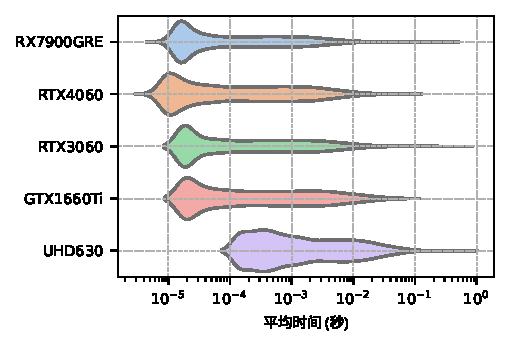
\includegraphics[width=0.8\linewidth]{figures/TimeMean.pdf}
    \caption{各 GPU 平台上性能样本关于时间的分布}
    \label{fig:archTimeMean_ch3}
  \end{figure}

\begin{figure}[h]
    \centering
    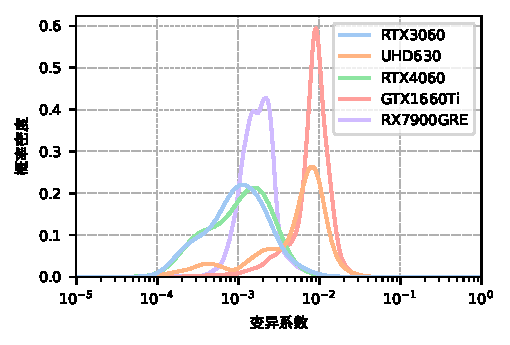
\includegraphics[width=0.8\linewidth]{figures/CV.pdf}
    \caption{各 GPU 平台上性能样本计算得到的变异系数分布}
    \label{fig:archTimeCV_ch3}
\end{figure}

\subsection{{\added 着色器性能挑战样本集}}

\label{sec:evaluation_challeng_shader}

{\added 图 \ref{fig:difficultSamples_ch3} 给出了着色器数据集中筛选出的挑战样本中随机抽样的 10 个样本,其在时间分布图上的关系。图中的红色线条代表其阶(或称序数)由图上方表示的平台到图下方表示的平台为上升趋势,绿色线条代表其阶由图上方表示的平台到图下方表示的平台为下降趋势。从图中可以同时看到,部分样本之间代表的线条出现了显著的交叉,这些交叉刻画了挑战样本的一类典型特征:在平台 A 上较另一着色器快的着色器,其在平台 B 上反而可能较慢。}

\begin{figure}[h]
    \centering
    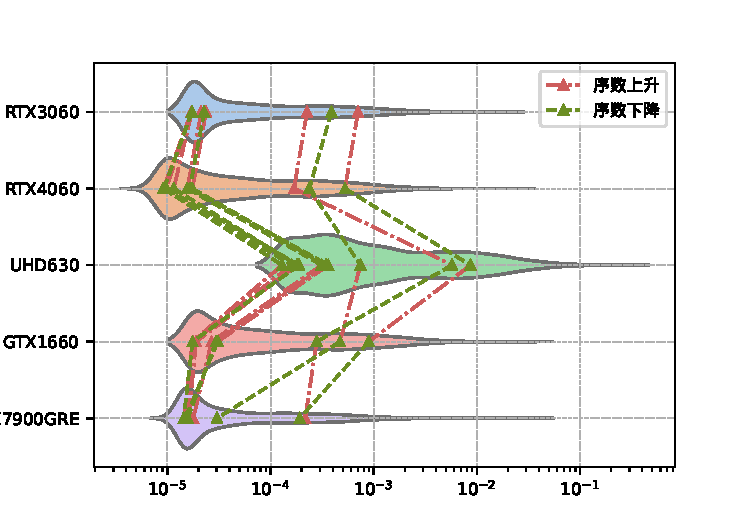
\includegraphics[width=0.8\linewidth]{figures/difficult.pdf}
    \caption{着色器性能挑战样本集抽样展示}
    \label{fig:difficultSamples_ch3}
\end{figure}

\subsection{{\added 着色器类型标注}}

{\added 在类型划分阶段,通过统计 Shadertoy 着色器中前 200 个标签,并经过人工筛选过滤和保守的标签等价关系推断后,形成了表 \ref{table:tag_classification} 所示的公共大类和所对应的用户提交标签的关系。大类共分为 8 个,其中 2d 和 3d 两类互斥,其余类别为满足特征时才需要部分或同时归属的类别。}

\begin{table}[h]
    \centering
    \caption{Shadertoy 经过类别划分后的公共大类和用户提交标签汇总}
    \label{table:tag_classification}
    \begin{tabular}{p{2cm}|p{11cm}}
        \toprule
        大类 & Shadertoy 子标签 \\
        \midrule
        2d & 2d \\
        3d & 4d, 3d \\
        raytracing & path, intersection, pathtracer, pathtracing, marching, raytrace, sdf, raytracing, raymarching, distancefield, distance, raymarcher, raymarch \\
        volume & volume, volumetric \\
        noise & perlin, bluenoise, noise, simplex, worley, fbm \\
        simulation & cellularautomata, reaction, particles, gameoflife, physics, diffusion, cellular, flow, simulation, automata, dynamics, fluid \\
        material & refraction, reflection, translucent, metal, mirror, water, transparency, glass, material, pbr, plastic \\
        effects & effect, feedback, blur, grain, convolution, distortion, dithering, dof, vignette, glitch, aberration, warp, bloom, postprocessing, glow, filter \\
        \bottomrule
    \end{tabular}
\end{table}

{\added 在监督样本标注阶段,本章共邀请了 3 名图形学领域的研究生同学,标注了共 156 个着色器样本的大类。这些着色器样本的大类的分布可以参考图 \ref{fig:manualLabelResultAndCVT_ch3}(a)。}

\begin{figure}[h]
    \centering
    \begin{minipage}[b]{\textwidth}
        \begin{subfigure}[b]{0.5\textwidth}
            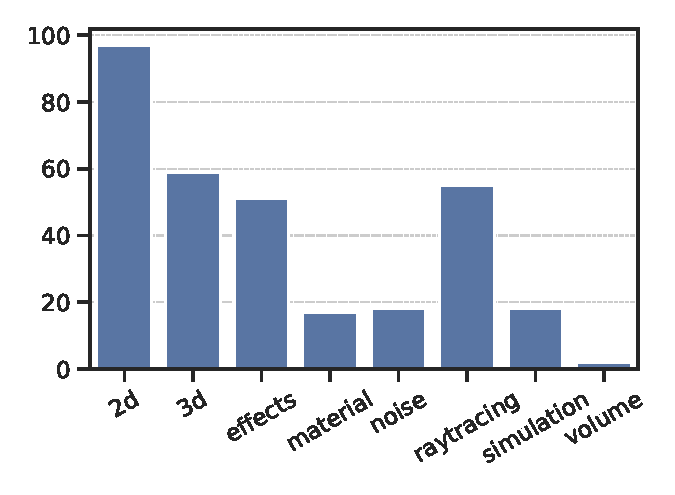
\includegraphics[width=\textwidth]{figures/ManualLabelResult.pdf}
            \caption{着色器监督样本大类分布}
        \end{subfigure}
        \begin{subfigure}[b]{0.5\textwidth}
            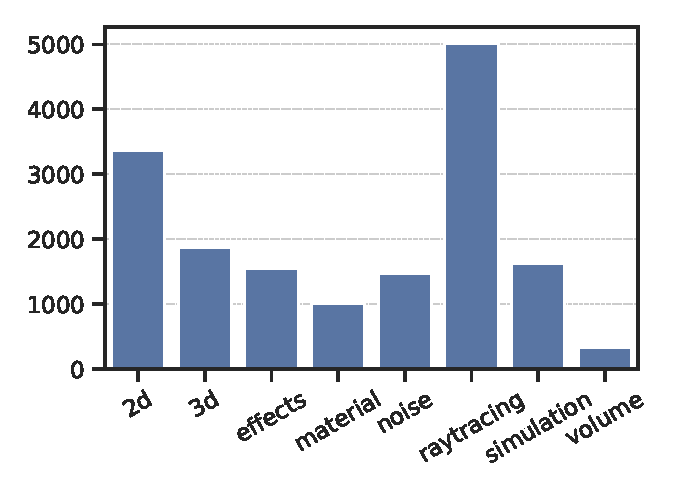
\includegraphics[width=\textwidth]{figures/AuthorLabel.pdf}
            \caption{着色器标签转换大类分布}
        \end{subfigure}
    \end{minipage}

    \caption{着色器样本大类分布情况一览}
    \label{fig:manualLabelResultAndCVT_ch3}
\end{figure}

{\added Shadertoy 子标签本身也可以映射到大类。然而,网站用户常常不会标记所有符合自己着色器的标签。如果假设每个用户均独立并以相同概率 $p$ 决定某个符合该作品内容的标签是否应该标记的话,那么就同样可以利用基于子标签转换的大类标签作为整个数据集分布的保守估计。这样转换得到的大类样本分布可以参考图 \ref{fig:manualLabelResultAndCVT_ch3}(b)。

将图 \ref{fig:manualLabelResultAndCVT_ch3}(a) 和图 \ref{fig:manualLabelResultAndCVT_ch3}(b) 联合比较可以看出,实际上不同标签被标注的喜好并不相同。例如,使用 raytracing 大类中标签的多为显示 3D 效果的着色器程序,但由着色器标签转换得到的大类分布中,3d 大类的绝对数量却小于 raytracing 标签的数量。这样的现象提示,直接使用原 Shadertoy 中的标签推测该着色器的类别是存在一定程度的误差的。

在大模型提示词探索阶段,本节选择了 3 种提示词写作方式,分别从没有类别的具体提示词、具有简单提示的提示词、具有比较详细提示的提示词三类出发,探究了提示词的写作对于分类性能的影响。三类提示词的具体构造可以参考附录 \ref{sec:prompt_appendix},其中较为详细的提示词相对于简单提示词中,主要增加了较为模糊的 noise,material 等几个标签的负例描述。同时,本文选择了来自 2 家大模型提供商的 4 种大语言模型,在监督数据集上进行了验证,验证结果如表 \ref{table:promptF1}。其中,{\bf qwen} 为阿里的通义千问大语言模型\cite{QWen},本节测试了其 turbo,plus 和 max 三个模型,三个模型的参数量依次递增。{\bf Baichuan2} 为百川智能的大语言模型\cite{Baichuan},本节测试了其 turbo 大模型。表中每类的最优表现以加粗字体显示。为了避免稀疏类别对整体效果评估的影响,本文在表格的最后一栏报告了各组的加权 F1 值。

从结果中可以得出如下几点结论。其一,分类表现受模型影响较大。qwen 的几个模型的表现整体均好于 Baichuan2 模型,而在最稠密的 2d、3d、raytracing、effects 几个标签中,qwen-max 的表现普遍好于 plus 和 turbo 模型。其二,对于 2d、3d 这对标识最基本的着色器特征,即着色器本身是否应用了 3D 渲染技术的类别标签,基座语言模型的标注已经基本可以满足需求。其三,部分类别的分类效果仍需要增强。material、noise 和 simulation 三个类别的分类效果在更换提示后改善并不明显。然而,在 2d、3d 类别中,从无类别提示到简单的类别提示的转换对于能力较强的模型起到了一定程度的效果。

}

\begin{table}[]
    \centering
    \caption{监督数据集上各组大模型在不同提示词下的分类 F1 表现}
    \label{table:promptF1}
    \resizebox{\textwidth}{!}{%
    \begin{tabular}{llllllllll|l}
        \toprule
        \multirow{2}{*}{提示类别}  & \multirow{2}{*}{模型名称} & \multicolumn{9}{c}{F1}                                                                                                                                          \\ \cline{3-11} 
        &                       & 2d              & 3d              & effects         & material        & noise           & raytracing      & simulation      & volume          & 加权     \\
        \midrule
        \multirow{4}{*}{无类别提示} & qwen-turbo      & 0.9082          & 0.8235          & 0.4252          & 0.2597          & \textbf{0.5098} & 0.8542          & 0.4000          & \textbf{1.0000} & 0.7197          \\
                               & qwen-plus       & 0.9326          & 0.8972          & 0.4198          & 0.2824          & 0.3469          & 0.8889          & \textbf{0.7222} & 0.4444          & 0.7528          \\
                               & qwen-max        & 0.9485          & 0.9020          & 0.5269          & 0.3333          & 0.4667          & 0.8750          & 0.5217          & 0.5714          & 0.7723          \\
                               & Baichuan2-Turbo & 0.8402          & 0.8174          & 0.4545          & 0.2500          & 0.4416          & 0.8421          & 0.4118          & 0.1667          & 0.6914          \\
        \midrule
        \multirow{4}{*}{简单提示}  & qwen-turbo      & 0.9061          & 0.8000          & 0.3673          & 0.3014          & 0.3500          & 0.8889          & 0.3600          & 0.5714          & 0.6996          \\
                               & qwen-plus       & 0.9271          & 0.8889          & 0.4354          & 0.3636          & 0.3301          & 0.8829          & 0.6122          & 0.1667          & 0.7464          \\
                               & qwen-max        & \textbf{0.9570} & \textbf{0.9184} & 0.5289          & 0.4444          & 0.3721          & 0.8776          & 0.4348          & 0.2857          & 0.7726          \\
                               & Baichuan2-Turbo & 0.8868          & 0.8333          & 0.5313          & 0.4000          & 0.3208          & 0.8305          & 0.4815          & 0.3077          & 0.7250          \\
        \midrule
        \multirow{4}{*}{详细提示}  & qwen-turbo      & 0.9290          & 0.8190          & 0.3860          & 0.3448          & 0.3836          & 0.8696          & 0.4490          & 0.2222          & 0.7168          \\
                               & qwen-plus       & 0.9091          & 0.8833          & 0.4769          & \textbf{0.4561} & 0.3579          & 0.8750          & 0.4889          & 0.1481          & 0.7446          \\
                               & qwen-max        & 0.9486          & \textbf{0.9184} & 0.4842          & 0.4186          & 0.4384          & \textbf{0.8936} & 0.4848          & 0.8000          & \textbf{0.7740} \\
                               & Baichuan2-Turbo & 0.8598          & 0.7619          & \textbf{0.5735} & 0.3810          & 0.3789          & 0.8430          & 0.4783          & 0.2857          & 0.7143          \\
        \bottomrule
        \end{tabular}%
    }
\end{table}

\section{{\added 本章小结}}

{\added 本章提出了面向性能预测的着色器性能数据集。首先,本章介绍了着色器程序数据集的收集和理解工作中面临的诸多挑战,并介绍了本章工作应对这些挑战的方面。之后,本章详细介绍了着色器收集和性能测量环节的具体实现、挑战样本集的构造,以及利用基座语言模型进行着色器类别标注的相关探索。最后,本章仔细分析了着色器数据集的分布特征,其受到其它因素所导致的性能波动的程度,着色器过滤和挑战样本的情况,以及基座语言模型对于类别标注问题的实践结果。}